\documentclass[a4paper, 10pt]{article}

\usepackage[utf8]{inputenc} % UTF-8 support
\usepackage{tikz} % for graph drawings

\title{Analysis of Algorithms Homework 2}
\author{Joseph Petitti}
\date{\today}

\begin{document}

\maketitle

\begin{enumerate}
	\item \begin{enumerate}
			\item Proof by induction:
				\begin{itemize}
					\item Base case: $n = 1$. In this case, you start with
						$v_1$ and give it color~1. $v_1$ has no adjacent
						vertices, so $G$ is legally colored.
					\item Inductive hypothesis: for all values of $n$ such that
						$n > 0$, the given algorithm legally colors $G$.
					\item Inductive step: $n = i + 1$. When the algorithm
						reaches the new node there are two possible cases:
						\begin{itemize}
							\item If $v_n$ can be legally colored by a
								previously used color, in which case assigning
								it a color is trivial.
							\item Otherwise, it can be assigned color~$i + 1$,
								which was not used in the previous graph with $n
								= i$ vertices.
						\end{itemize}
				\end{itemize}

			\item The algorithm runs in $O(n^2)$ time. Proof:
				\begin{itemize}
					\item The algorithm must iterate through each node $v_1
						\dots v_n$. This gives it at least linear time.
					\item For each node $v_i$, the algorithm iterates through
						each of its neighbors in $\{ v_1 \dots v_{i-1} \}$. In
						the worst case, each node $v_i$ has $i-1$ such
						neighbors. This gives us a worst-case time complexity of
						$O(n (n - 1))$, which simplifies to $O(n^2)$.
				\end{itemize}

			\item Because the algorithm uses the minimum color out of $\{ 1
				\dots n \}$, it always prefers to reuse a color rather than pick
				an unused one. At any node, $v_i$, with degree $d$, the
				highest color the algorithm will pick is $d + 1$, in the case
				where all of $v_i$'s neighbors are already colored with unique
				colors. Therefore, the highest color the algorithm can pick is
				the maximum degree plus 1.

				\begin{figure}[h]
					\centering
					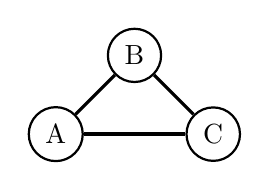
\begin{tikzpicture}[every node/.style={circle,thick,draw},
										every edge/.style={very thick,draw}]
						\node (A) at (0, 0) {A};
						\node (B) at (1, 1) {B};
						\path [-] (A) edge (B);
						\node (C) at (2, 0) {C};
						\path [-] (B) edge (C);
						\path [-] (A) edge (C);
					\end{tikzpicture}
				\end{figure}

				In the  graph above, $\Delta$, the maximum degree of a vertex,
				is 2. Assume the algorithm decides to traverse the vertices in
				the order $A$, then $C$, then $B$. At node $A$, it sees that
				none of $A$'s neighbors are already colored, so assigns it color
				1. At $C$, it sees that the neighbor $A$ is already assigned
				color~1, so it assigns $C$ the next lowest color, 2. At node
				$B$, it sees that neighbors $A$ and $B$ already have the colors
				1 and 2, respectively, so assigns it the next lowest color
				color, 3. In this graph, 3 colors are used, which is equal to
				$\Delta + 1$.

			\item 
		\end{enumerate}

	\item To solve this problem, use a modified version of Kruskal's algorithm.
		Start with edge $e$ in your MST. Sort the remaining edges in order of
		weight. Then, go through the edges in order from smallest weight to
		largest, and add each to the minimum spanning tree if it it attached to
		a vertex that is not already in the minimum spanning tree. The time
		complexity is $O(|E| \log |V|)$. Sorting the edges with comparison sort
		takes $O(|E| \log |E|)$ time, and allows you to remove the minimum
		element in constant time.

		Proof of correctness:

		\begin{itemize}
			\item Let $T$ be the spanning tree generated by the algorithm above,
				and $T'$ be a minimum cost spanning tree of $G$ that contains
				$e$.
			\item Assume that $T$ and $T'$ do not have the same set of edges.
			\item Let $h$ be a minimum cost edge such that $h \in E(T)$ but $h
				\notin E(T')$.
			\item If $h$ were included in $T'$ it would create a cycle. Because
				$T$ has no cycles, one of the edges in the cycle must not be in
				$T$. Call this edge $i$.
			\item If the weight of $i$ was less than the weight of $h$, it would
				have been selected by the algorithm first and included in $T$.
				Therefore $w(i) \ge w(h)$.
			\item Remove $i$ from $T'$ and add $h$ to it. This breaks the cycle
				without  increasing the total cost of $T'$, because $w(h) \le
				w(i)$.
			\item Repeat this for every edge $j$ such that $j \in E(T)$ but $j
				\notin E(T')$. $T'$ is now converted into $T$ without increasing
				the cost.
			\item Therefore $T$ is optimal.
		\end{itemize}

	\item $G$ is the graph below, $s$ is node $B$. In the graph below, the
		shortest path tree rooted in $B$ is the edges $(B, A)$ and $(B, C)$.
		However, the minimal spanning tree is $\{ (A, B), (A, C) \}$.
		\begin{figure}[h]
			\centering
			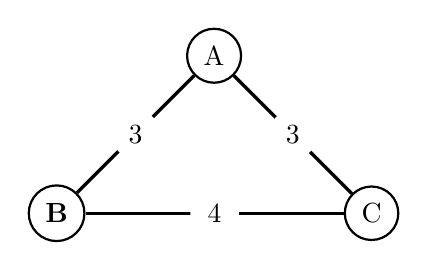
\begin{tikzpicture}[every node/.style={circle,thick,draw}]
				\node (A) at (2, 2) {A};
				\node (B) at (0, 0) {\textbf{B}};
				\node (C) at (4, 0) {C};

				\begin{scope}[every node/.style={fill=white,circle},
					          every edge/.style={draw,very thick}]
					\path [-] (A) edge node {$3$} (B);
					\path [-] (C) edge node {$3$} (A);
					\path [-] (B) edge node {$4$} (C);
				\end{scope}
			\end{tikzpicture}
		\end{figure}

	\item \textbf{Algorithm}:
		\begin{itemize}
			\item Add a vertex $s$ to $G$ such that $s$ is connected to every
				vertex in $S$ by an edge with weight 0. Similarly, add a vertex
				$t$ to $G$ such that $t$ is connected to every vertex in $T$ by
				an edge with weight 0.
			\item Now we only need to find the shortest path between $s$ and
				$t$. Dijkstra's algorithm can do this. This algorithm is
				explained on page 138 of Kleinberg and Tardos's ``Algorithm
				Design.''
			\item Now that we have the shortest path between $s$ and $t$, call
				that set of nodes $P$.
			\item Remove $s$ and $t$ from $P$. The result is the shortest path
				connecting a vertex in $S$ to a vertex in $P$.
		\end{itemize}

		\textbf{Time complexity}: Adding $s$ and $t$ takes $O(\max (|S|, |T|))$
		time. Dijkstra's algorithm takes $O(|E| + |V| \log |V|)$ when using a
		Fibonacci Heap and adjacency list. The final step takes constant time.
		This simplifies to $O(|E| + |V| \log |V|)$, which is the same as
		Dijkstra's algorithm.

		\textbf{Proof of correctness}: By the definition of Dijkstra's
		algorithm, the algorithm will return a correct shortest path between $s$
		and $t$. By adding $s$ and $t$ to the graph with 0-weight paths to every
		node in $S$ and $T$ respectively, Dijkstra's algorithm look for a
		shortest path that connects $s$ to $t$ by passing through both $S$ and
		$T$.
\end{enumerate}

\end{document}

